\documentclass{article}

\usepackage[a4paper, total={6.5in, 11in}]{geometry}
\setlength{\parindent}{0em}

\usepackage{latex/common}

\usepackage{graphicx}
\graphicspath{{titech/CSC.T433.AdvancedComputerArchitecture/final/}}

\title{ACA - Final}
\author{Sixue Wang \\ 21M30927}

\begin{document}

\maketitle

\section{}
V-Way cache wants to fill the gap between processor speed and main-memory access latency.
Reducing miss rate is one of the most significant methods if the cache size is fixed.
In the classic cache placement policies, fully associative cache can achieve the minimum miss rate but requires more power consumption and overhead.
Actually, it benefits from the maximum associativity and the global replacement strategy, exactly the set-associative cache lacks.
The disadvantage of set-associative cache is that data line can only be mapped to tag in the same set.
Unfortunately, this disadvantage could be magnified because program access memory non-uniformly, causing some sets to be overload but some to be underload.
V-Way cache can improve set-associative cache by increasing associativity and using global replacement but with less overhead than fully associative cache.
It doubles tag-store size and decouples tag-store and data-store which allows any data line to be mapped by any tag, even in a different set.
The operation of V-Way cache has two situation:
1) there is not enough number of tags in the current set then replace locally;
2) there is at least one empty tag then replace globally.
And the paper also proposed a new globally replacement algorithm based on the reuse counter. This algorithm requires less storage and computation cost because the bit of counter is 2 typically. But this algorithm has one obvious shortcomings which is the stronge assumption based on secondary cache.

\section{}
I use ``beq'' and ``j'' to implement loop. I also insert some ``nop'' to solve data dependency, branch, and jump. For machine code, please refer the verilog code.
\subsection{}
\lstinputlisting[basicstyle=\ttfamily,
                 title=code1.s]{titech/CSC.T433.AdvancedComputerArchitecture/final/code1.s}
\subsection{}
\lstinputlisting[basicstyle=\ttfamily,
                 title=code2.s]{titech/CSC.T433.AdvancedComputerArchitecture/final/code2.s}
\section{}
\subsection{}
I implemented ``add'', ``addi'', ``lw'', ``sw'', ``beq'', ``bne'', and ``j'', but I don't use ``bne'' in our assembly code.

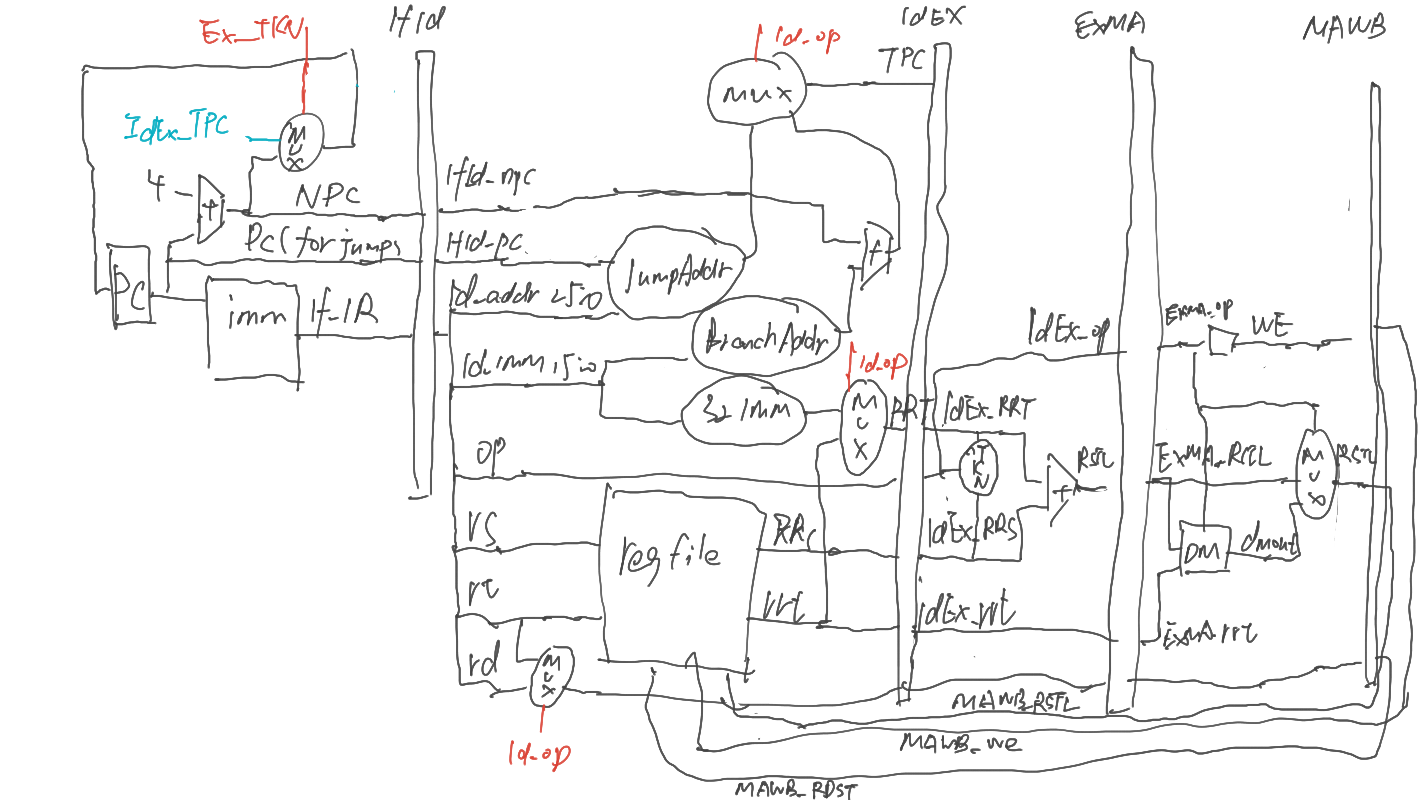
\includegraphics[width=\textwidth]{diagram}

\subsection{}
I only show ``code2.v'' in this pdf. The difference between ``code1.v'' and ``code2.v'' is the machine code of assembly code. You can find ``code1.v'' in the zip file.
\lstinputlisting[title=code2.v]{titech/CSC.T433.AdvancedComputerArchitecture/final/code2.v}

\subsection{}
To be simple, I change 100 to 1 for code1 and change 200 to 3 for code2. I only show the overall and the final result screenshot of waveforms. You can find the following vcd files in zip file.
\begin{itemize}
  \item ``code1-100.vcd'': original code
  \item ``code1-1.vcd'': 100 to 1
  \item ``code2-200.vcd'': original code
  \item ``code2-3.vcd'': 200 to 3
\end{itemize}

\subsection{}
Screenshot:

code1, 100 to 1, overall

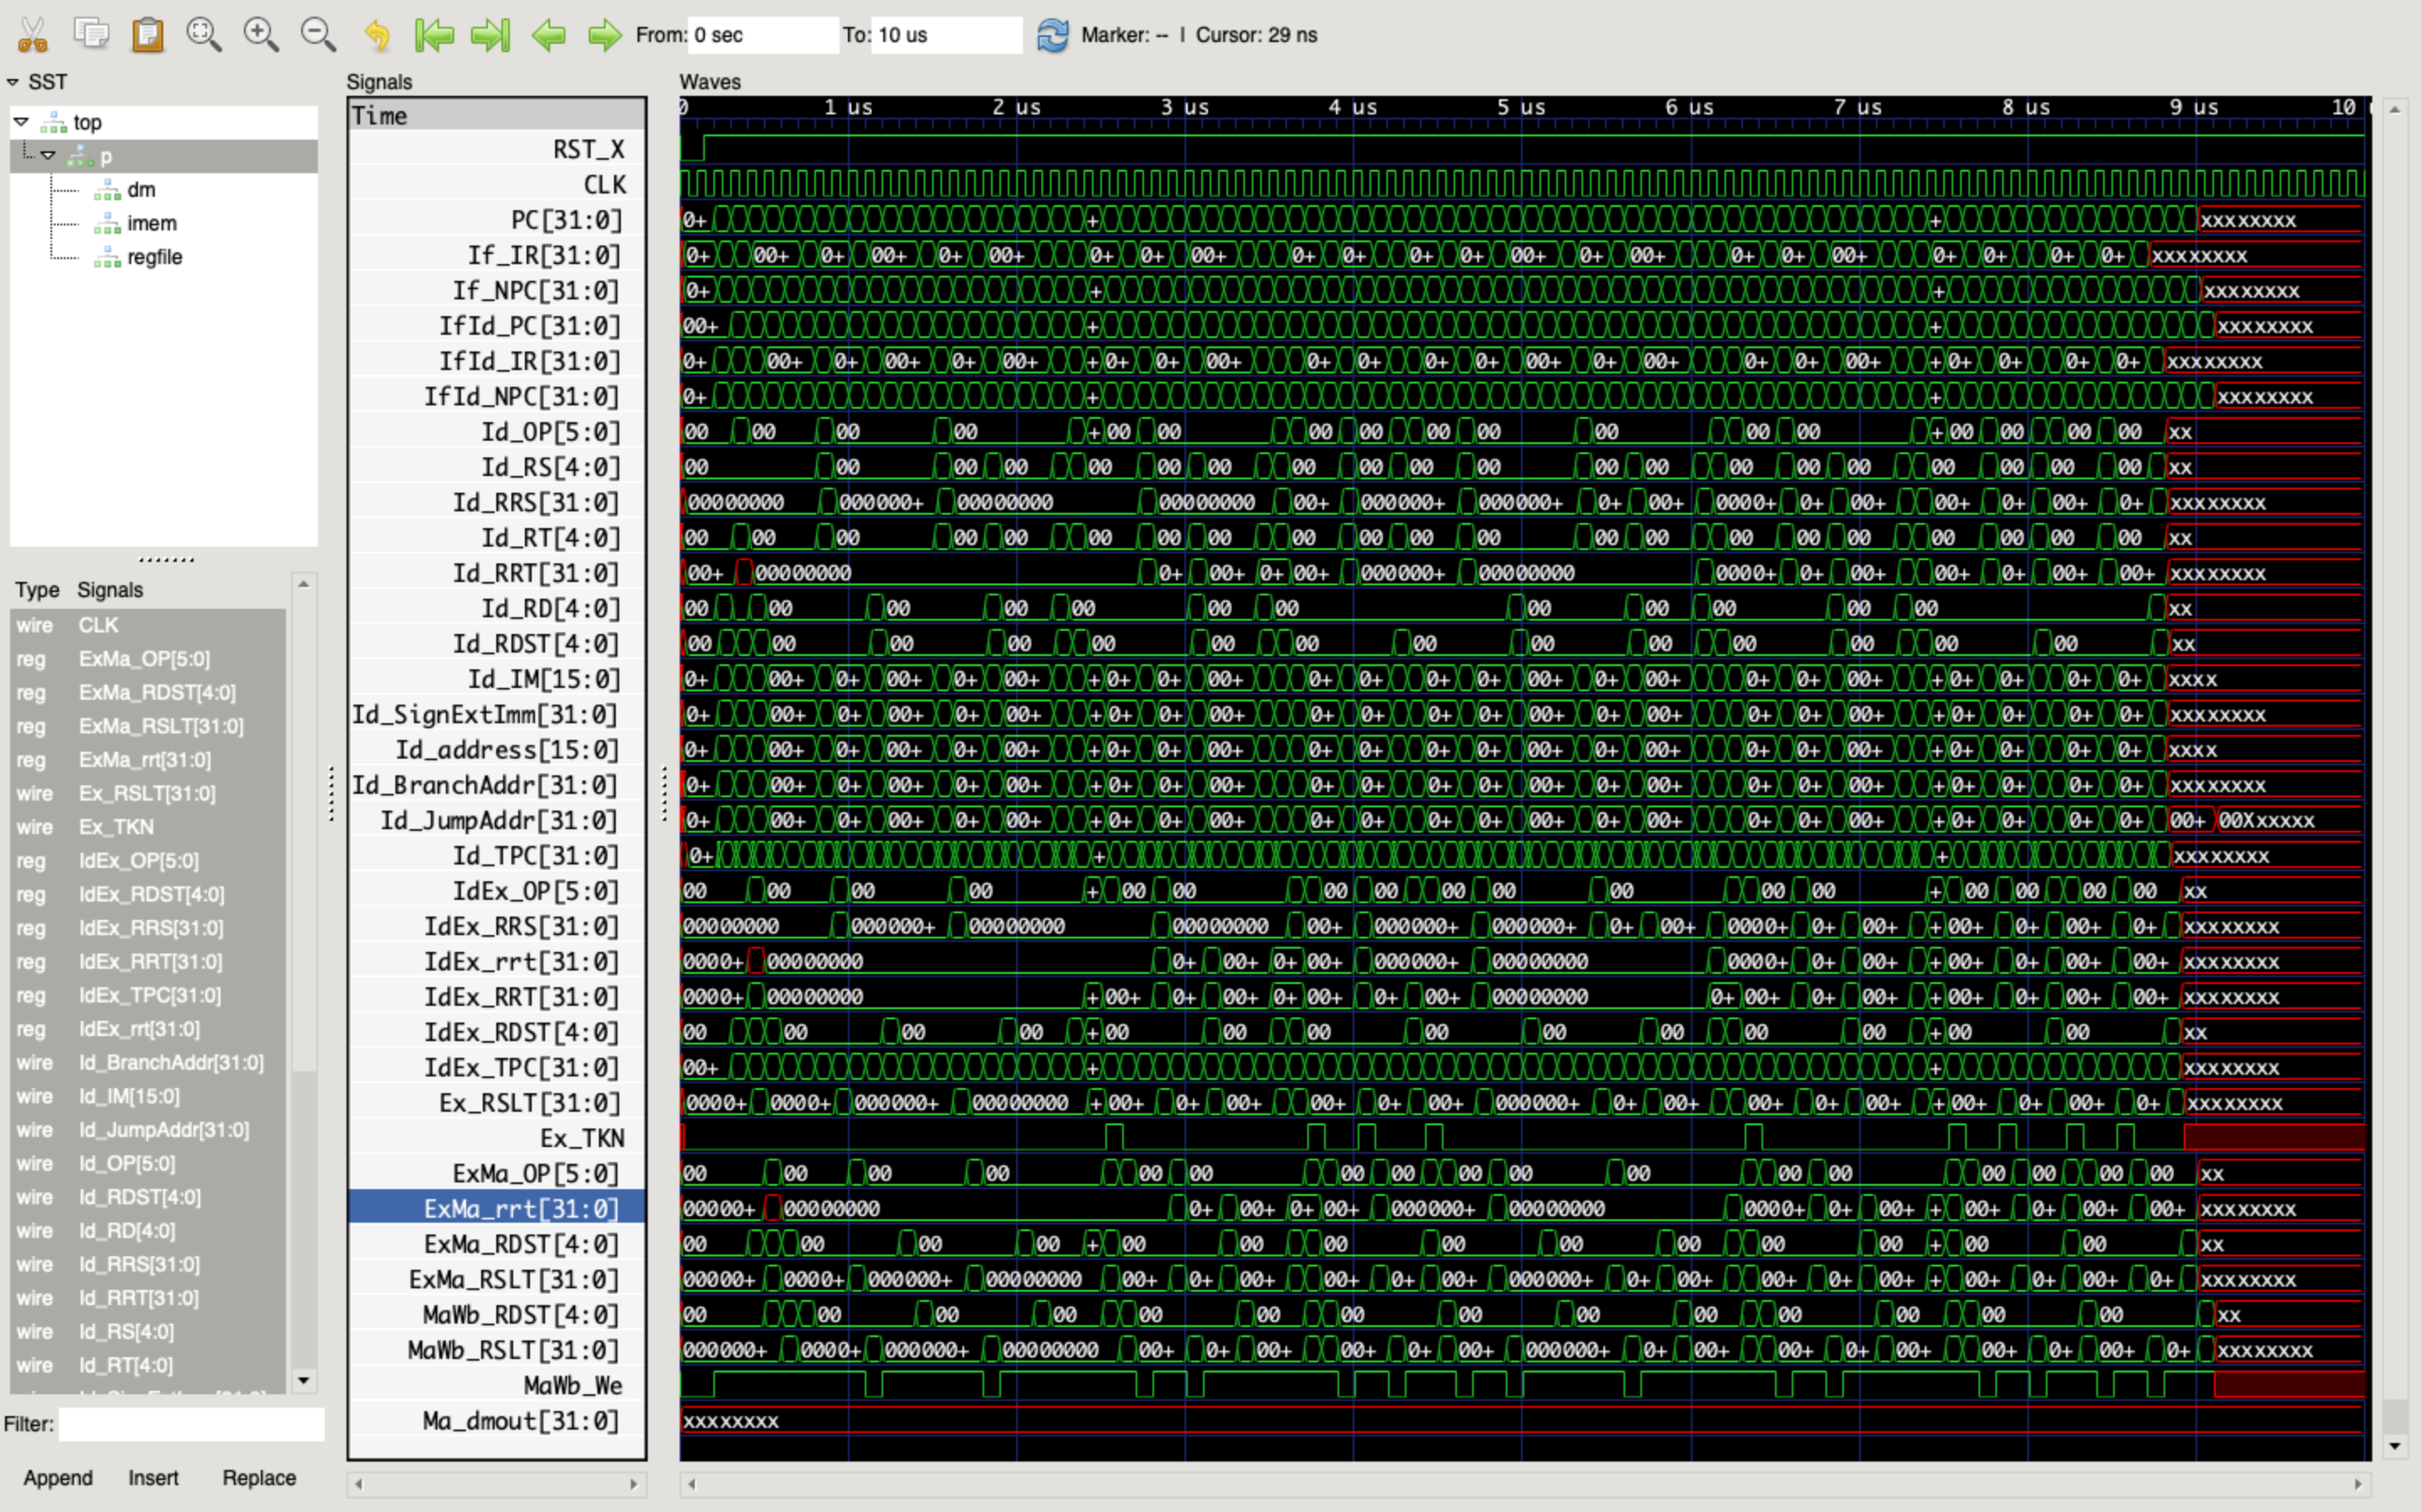
\includegraphics[width=\textwidth]{code1-1-0.png}

code1, 100 to 1, result

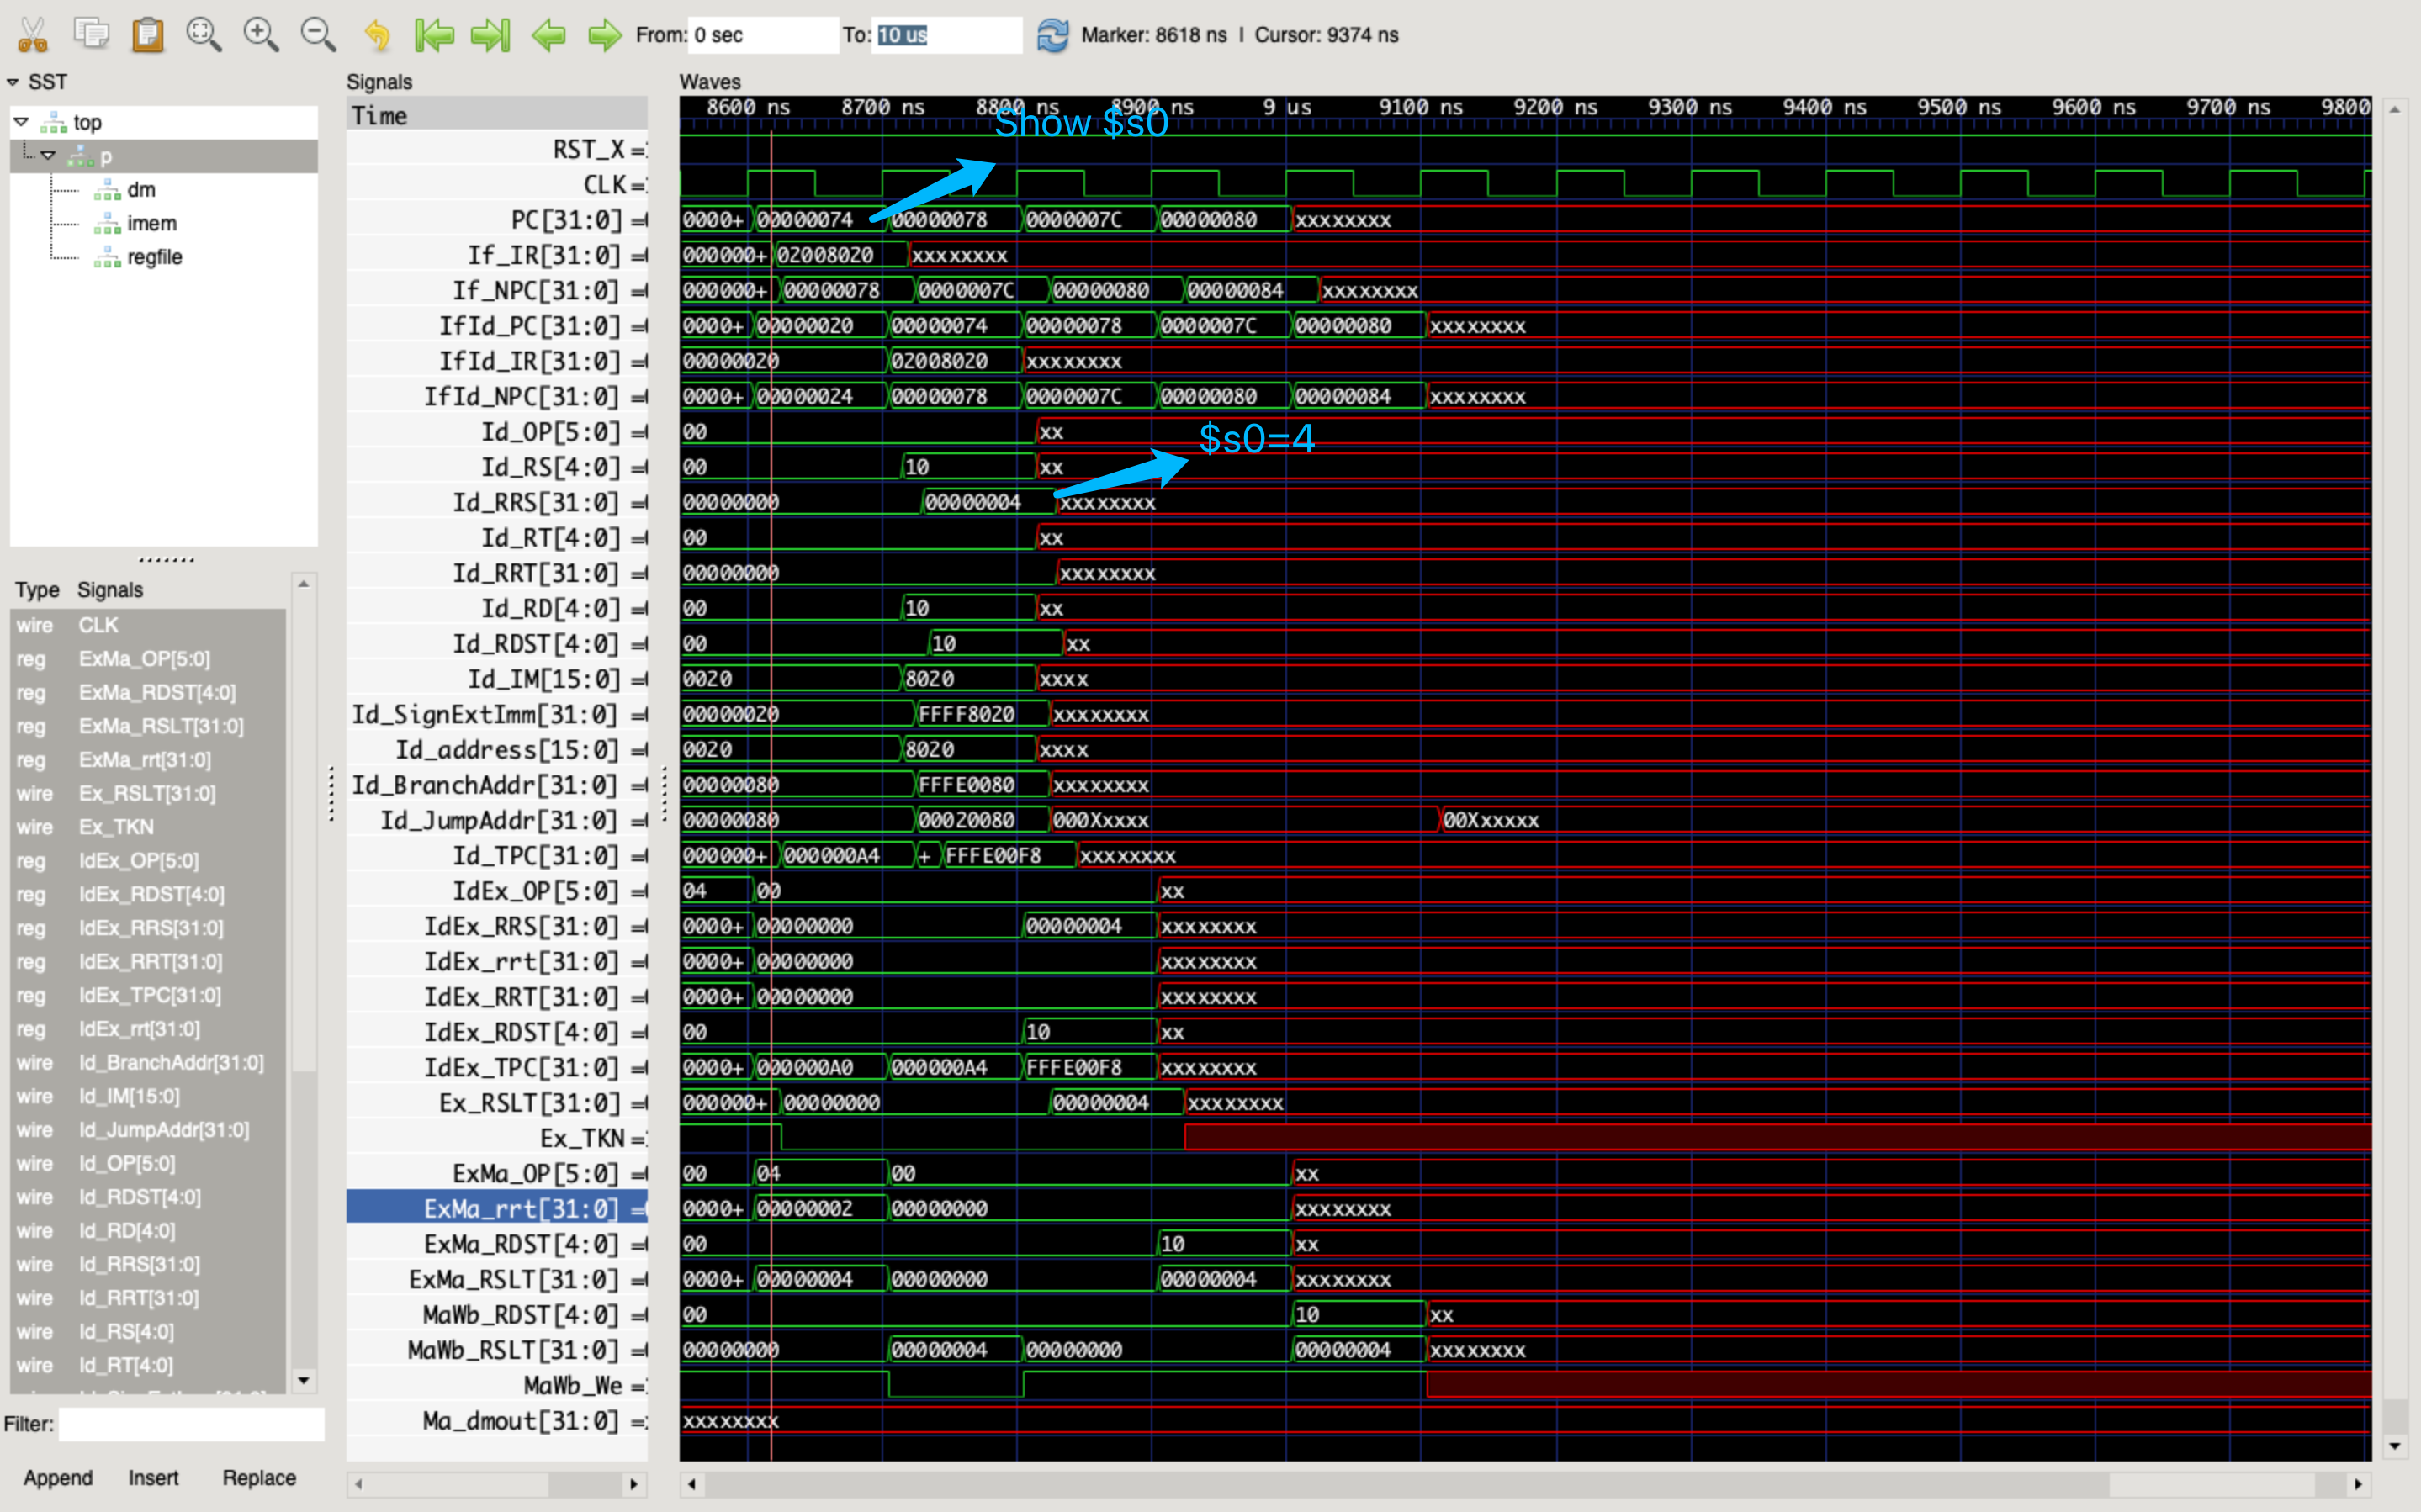
\includegraphics[width=\textwidth]{code1-1-1.png}

code2, 200 to 3, overall

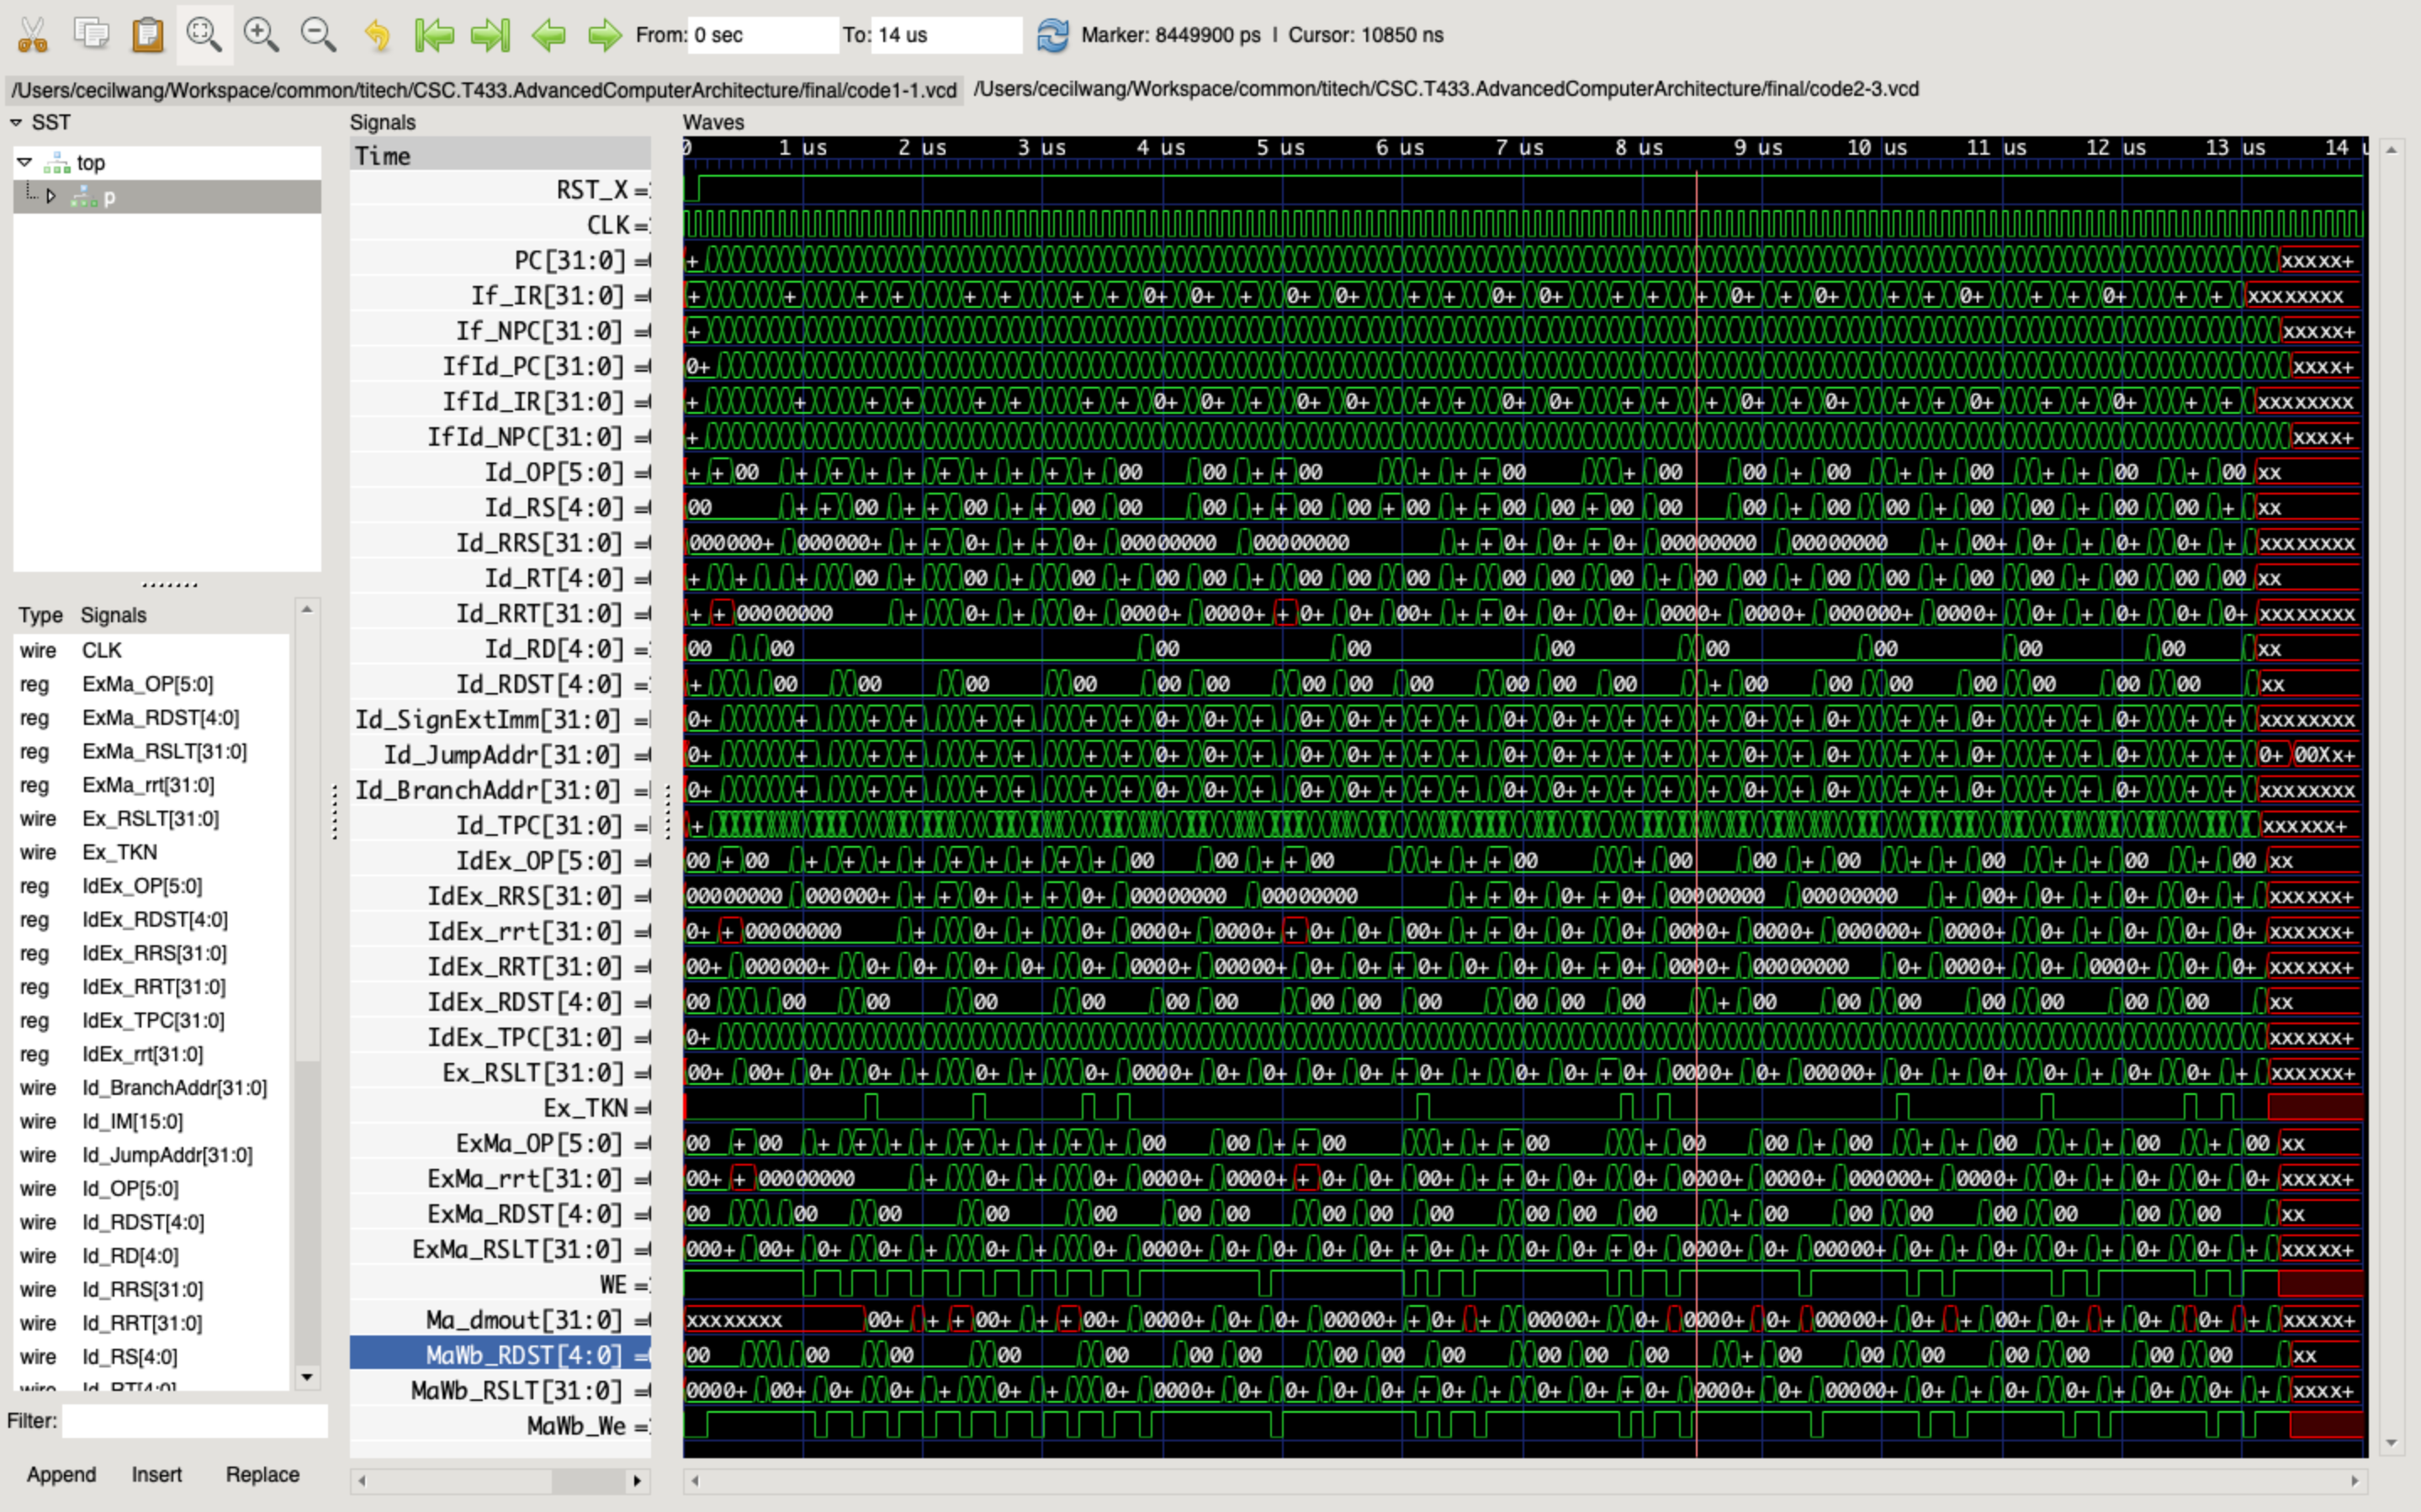
\includegraphics[width=\textwidth]{code2-3-0.png}

code2, 200 to 3, result

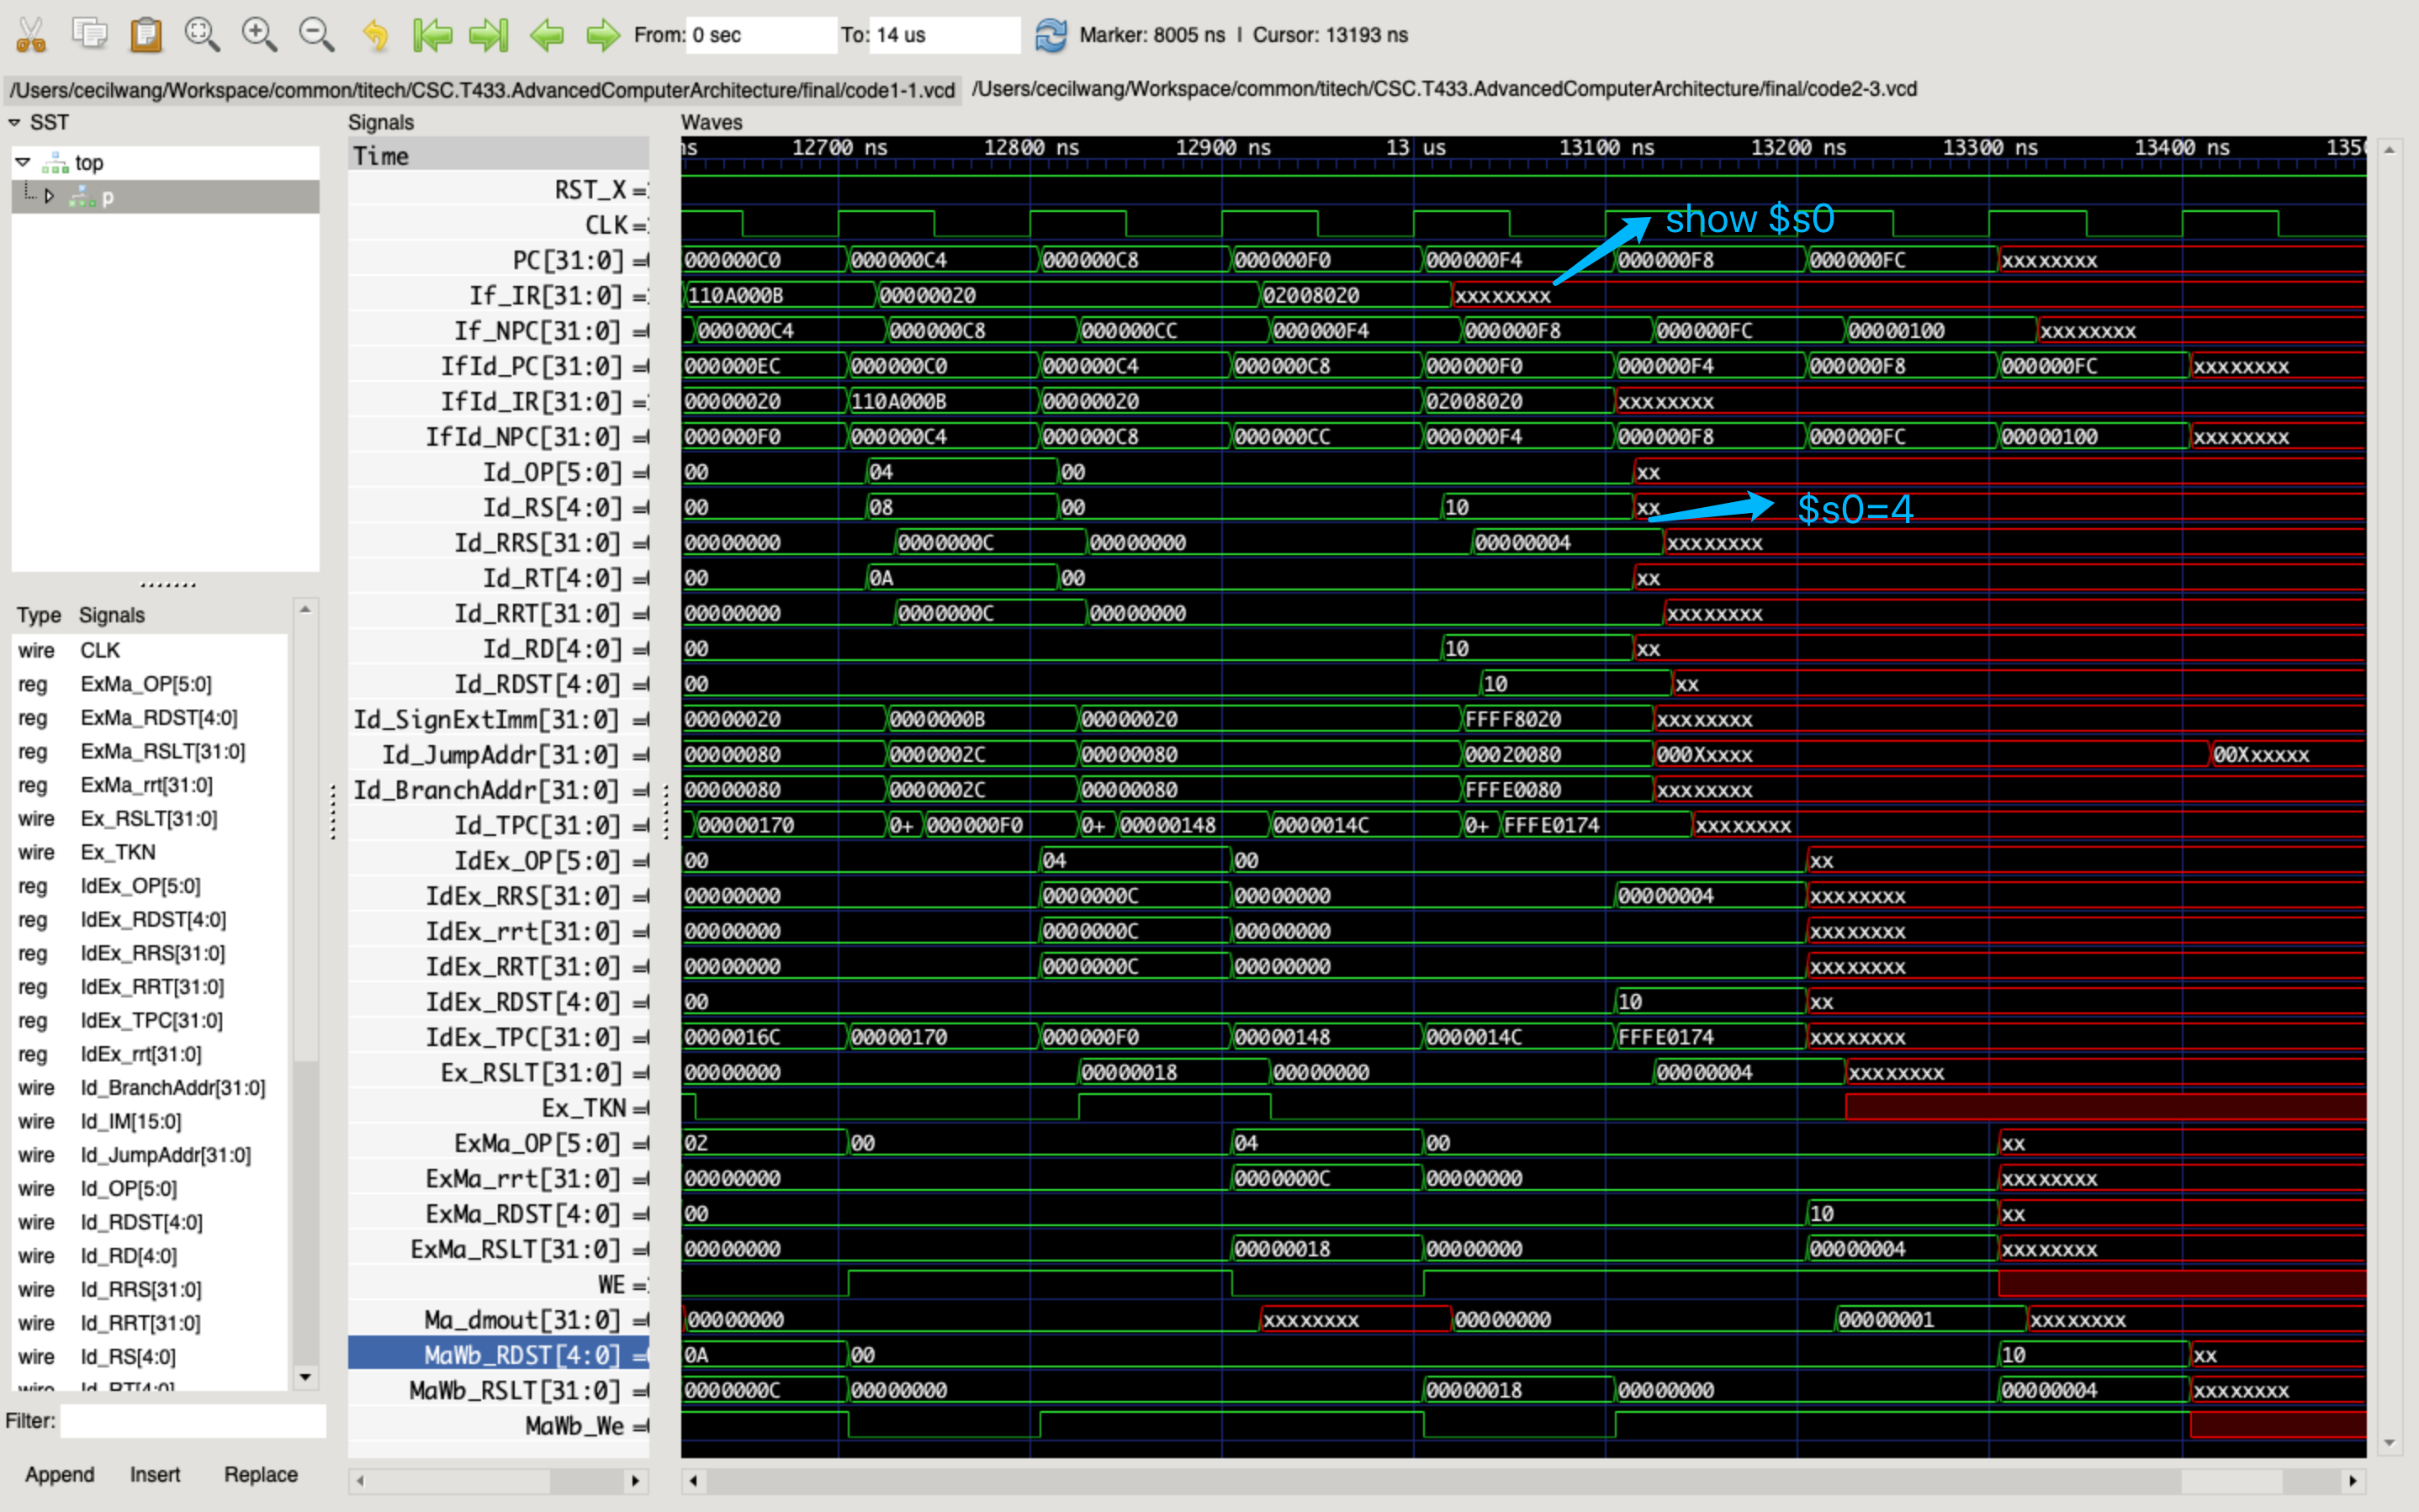
\includegraphics[width=\textwidth]{code2-3-1.png}

\section{}
\subsection{}
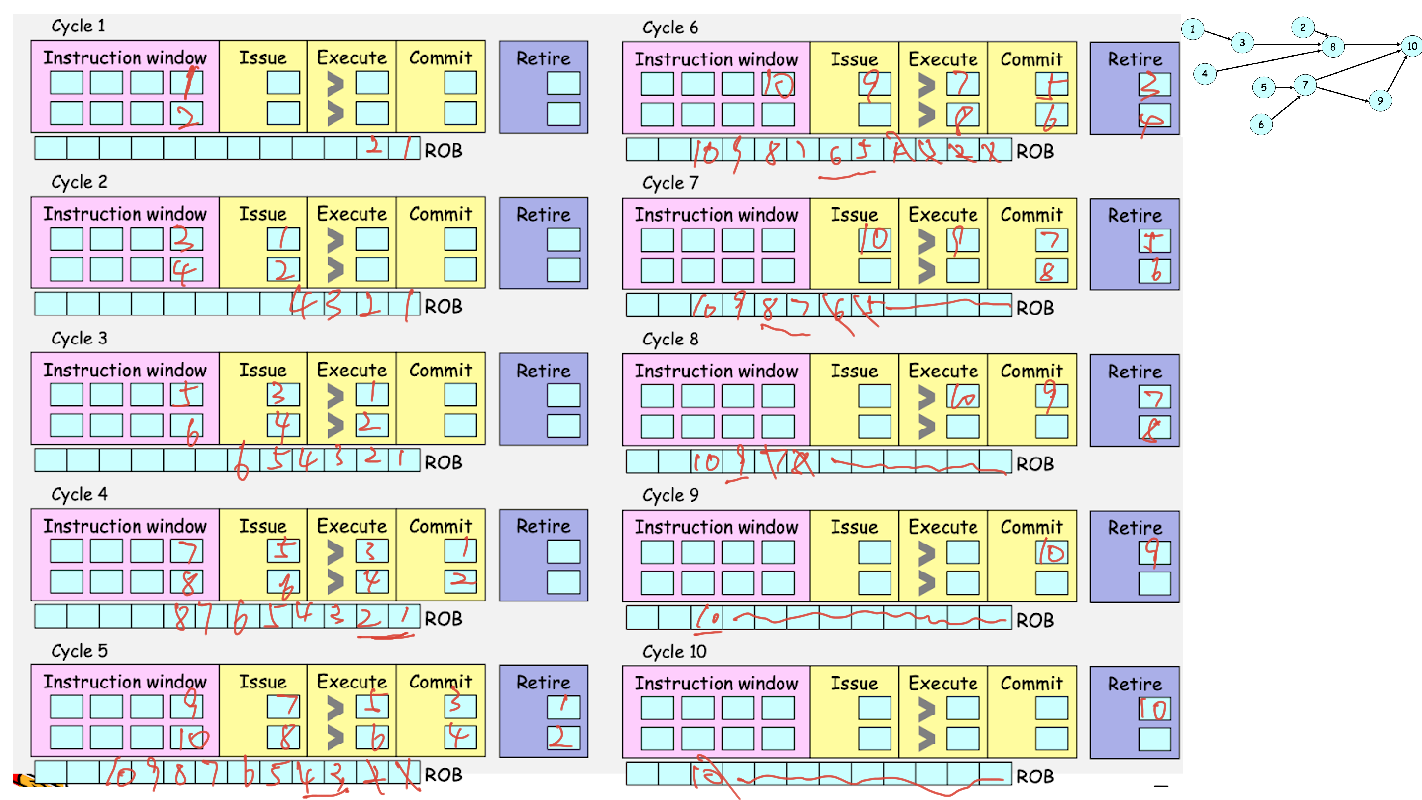
\includegraphics[width=\textwidth]{cycle10-1.png}
\subsection{}
I omit the final trivial cycle.

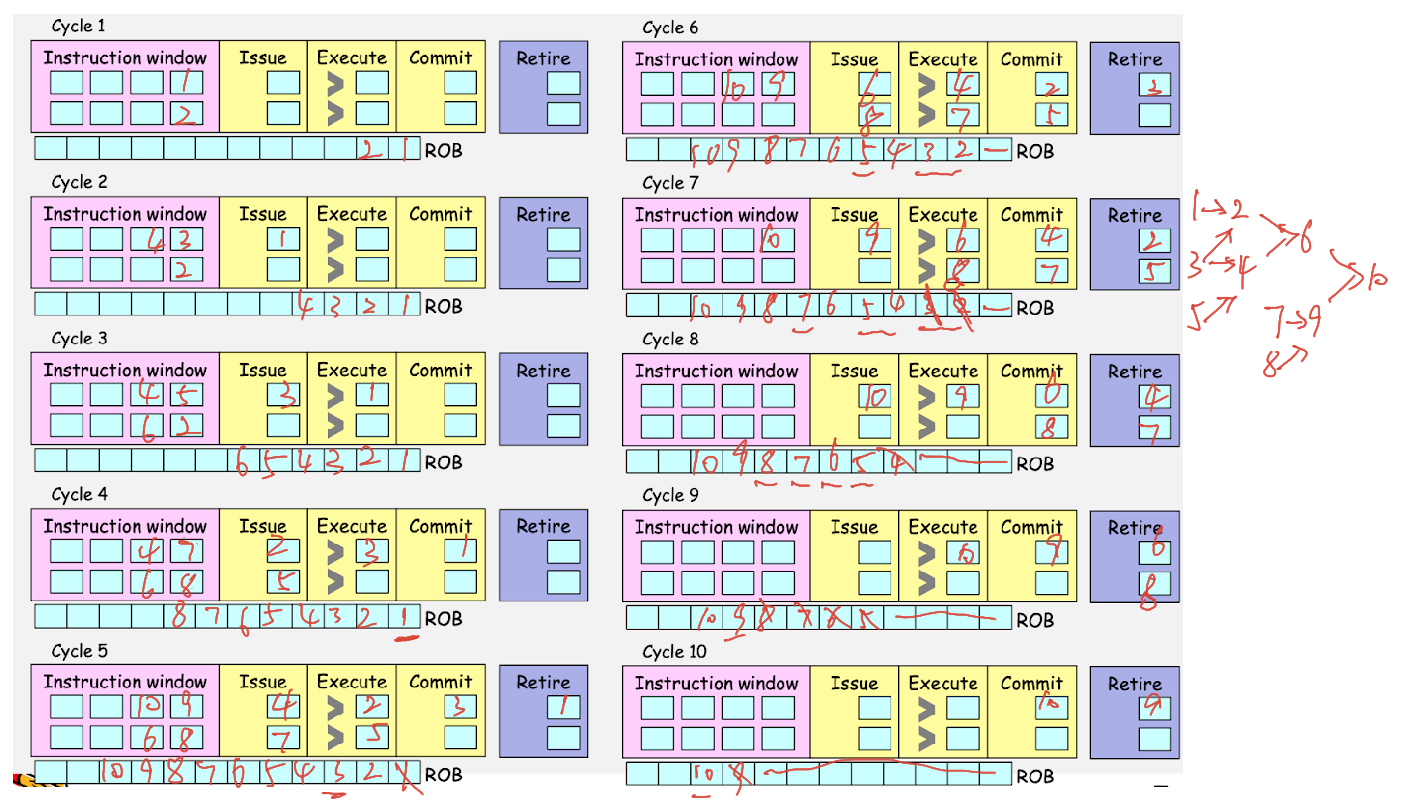
\includegraphics[width=\textwidth]{cycle10-2.png}

\section{}
\lstinputlisting[language=C++,
                 basicstyle=\ttfamily,
                 keywordstyle=\color{blue}\ttfamily,
                 commentstyle=\color{green}\ttfamily,
                 escapeinside={@}{@},
                 title=parallel\_solve.cc]{titech/CSC.T433.AdvancedComputerArchitecture/final/parallel.cc}

Basically, all loops in the original implementation were divided into ``NCORES'' threads to handle. These loops can theoretically be sped up ``NCORES'' times, but with a little overhead, such as post-loop synchronization.

Correctness can be guaranteed by adding locks or barriers when updating shared data or keeping shared status(diff, boundary: ``A[mymin], A[mymax], B[mymin], B[mymax]''). I comment reasons for all locks and barriers in the code.

\section{}
\lstinputlisting[basicstyle=\ttfamily,
                 title=fai.s]{titech/CSC.T433.AdvancedComputerArchitecture/final/fai.s}
\lstinputlisting[basicstyle=\ttfamily,
                 title=barrier.cc]{titech/CSC.T433.AdvancedComputerArchitecture/final/barrier.cc}

\section{}
The cpu of my pc is ``1.1 GHz Quad-Core Intel Core i5'':
\begin{itemize}
  \item cache line : 64byte
  \item 8 way set associative cache
  \item write-back and write allocate
  \item L1 icache  : 4KB
  \item L1 dcache  : 6KB
  \item L2         : 64KB
  \item L3         : 768KB
  \item Main Memory: 8GB
\end{itemize}
The cache coherence prototol is MESIF.\footnote{https://en.wikipedia.org/wiki/MESIF\_protocol} It consists of five states:
\begin{itemize}
  \item Modified: cache line is only stored in current cache and should be written back to main memory
  \item Exclusive: cache line is only stored in current cache and is same with main memory
  \item Shared: cache line may be stored in other caches and is same with main memory
  \item Invalid: cache line is invalid
  \item Forward: cache should act as a designated responder for any requests for the given cache line
\end{itemize}
In case of MESIF, a cache line request will be responded to only by the cache holding the line in the F state.


\end{document}
